\chapter{Исследовательская часть}

\section{Среда для тестирования}

Для тестирования разработанного алгоритма применялась облачная платформа Google Colab, не требующая установки ПО на локальный компьютер.

% 

\section{Проверка статистических гипотез}

\begin{figure}
	\begin{center}
		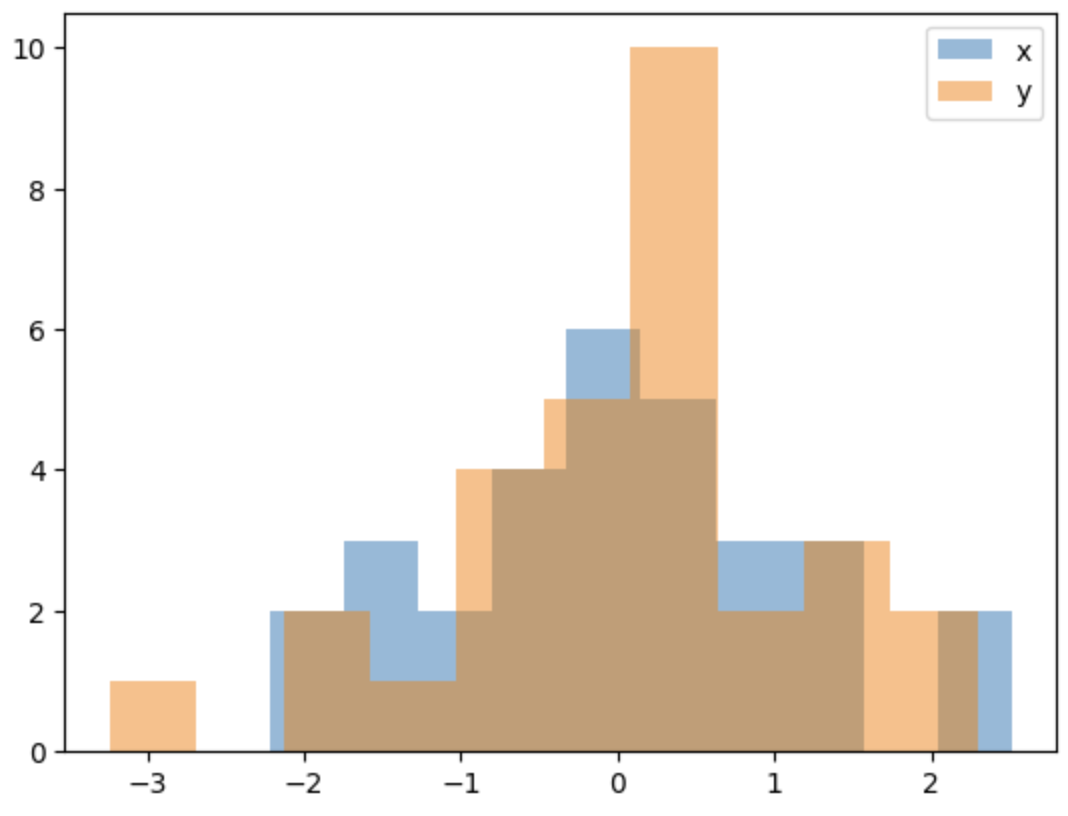
\includegraphics[width=0.75\textwidth]{images/1.png}
	\end{center}
	\caption{Исходные данные}
	\label{img:1}
\end{figure}

\begin{figure}
	\begin{center}
		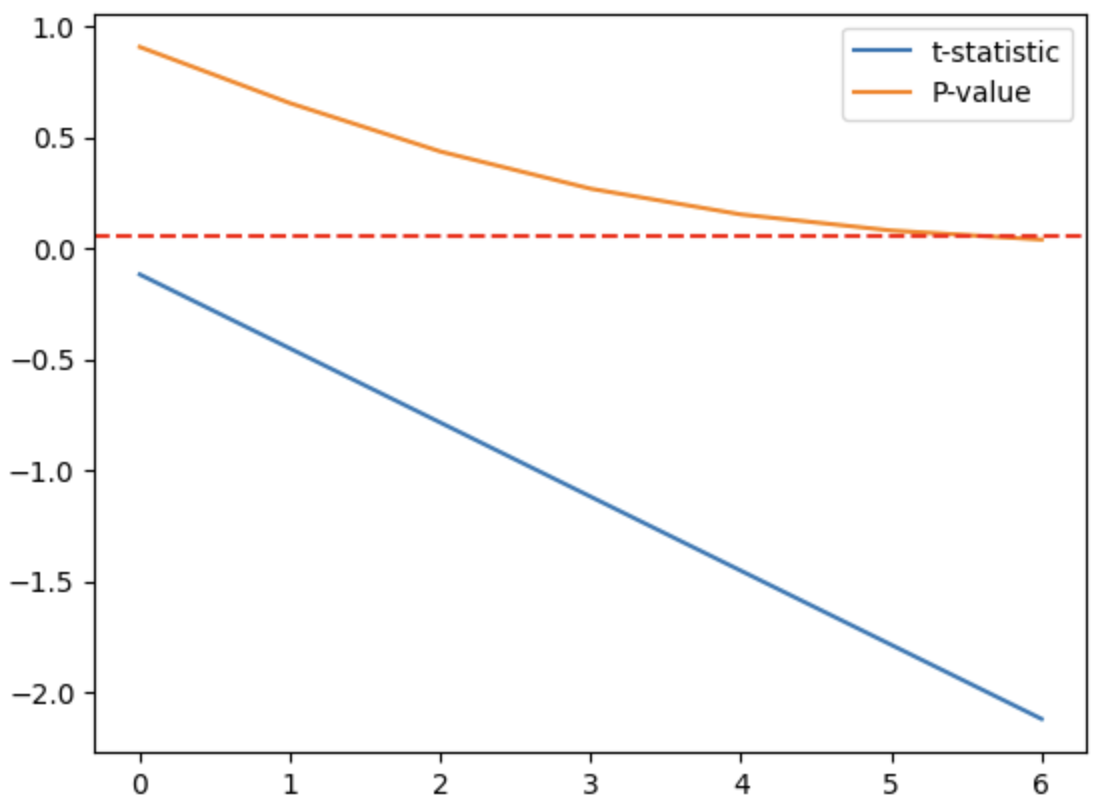
\includegraphics[width=0.75\textwidth]{images/2.png}
	\end{center}
	\caption{Динамика изменения значений статистики критерия и P-value для всех итераций проверки гипотезы о мат. ожидании при смещении второй выборки}
	\label{img:2}
\end{figure}

\begin{figure}
	\begin{center}
		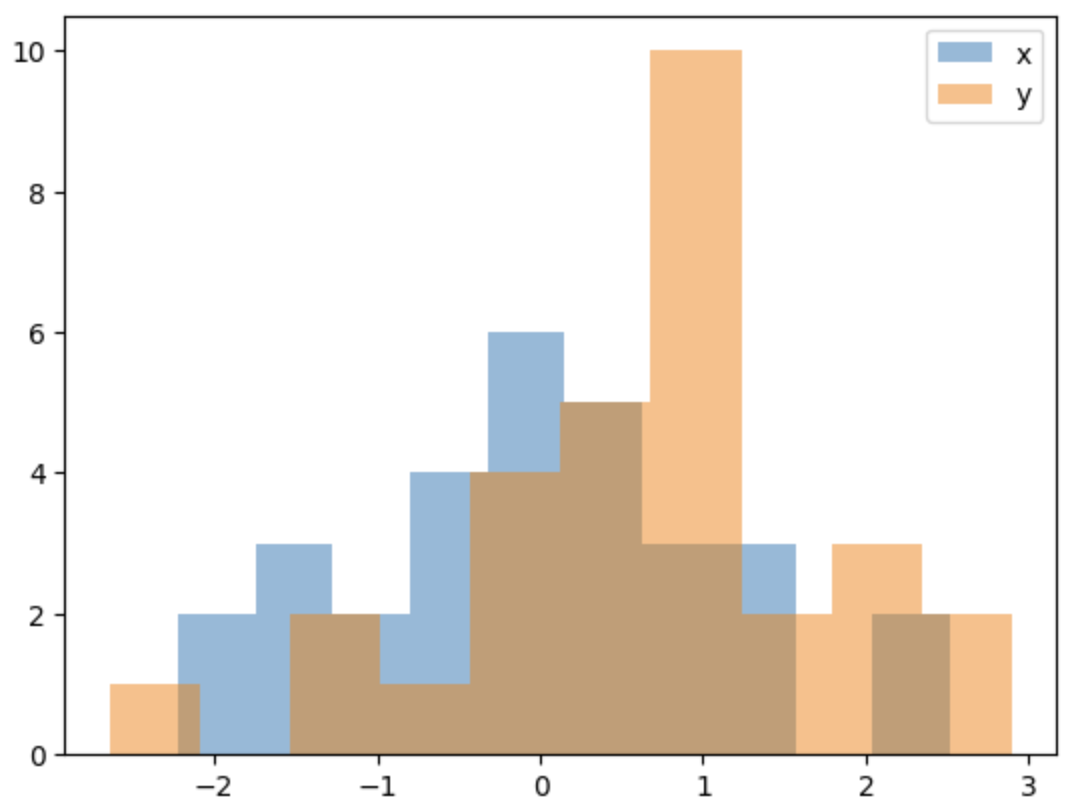
\includegraphics[width=0.75\textwidth]{images/3.png}
	\end{center}
	\caption{Выборки в момент, когда гипотеза была отвергнута}
	\label{img:3}
\end{figure}

\begin{figure}
	\begin{center}
		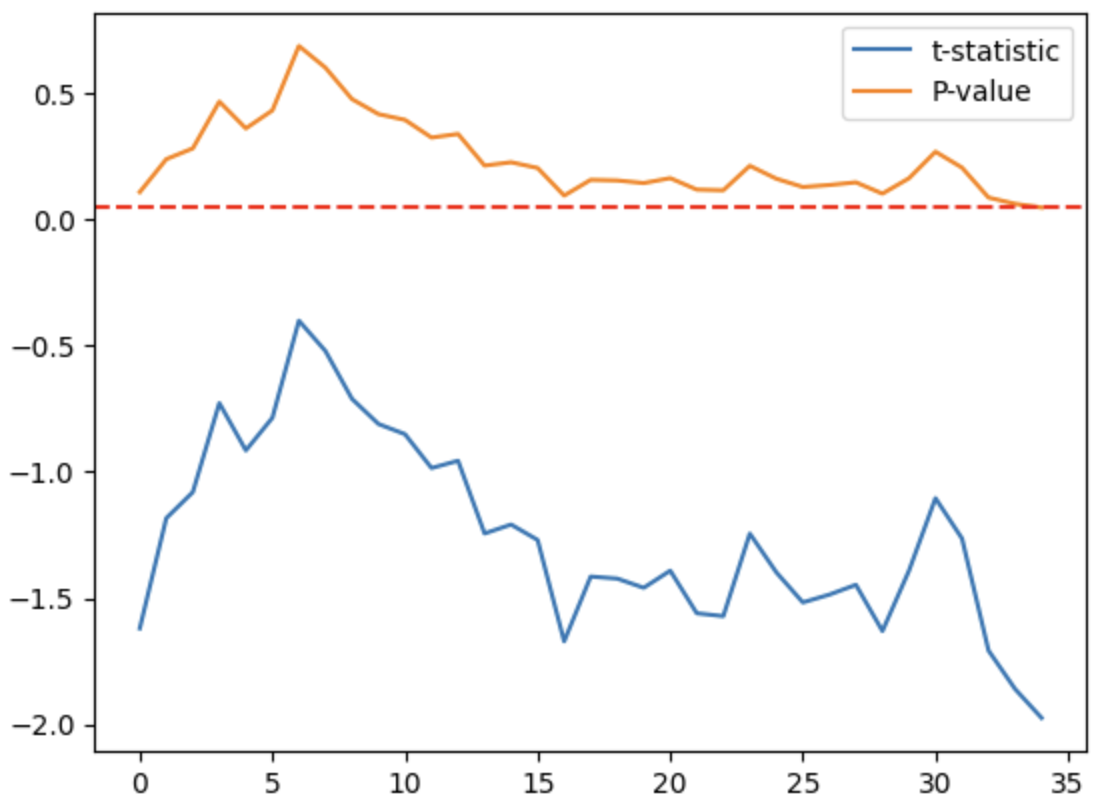
\includegraphics[width=0.75\textwidth]{images/4.png}
	\end{center}
	\caption{Динамика изменения значений статистики критерия и P-value для всех итераций проверки гипотезы о мат. ожидании при увеличении объёмов выборок}
	\label{img:4}
\end{figure}

\begin{figure}
	\begin{center}
		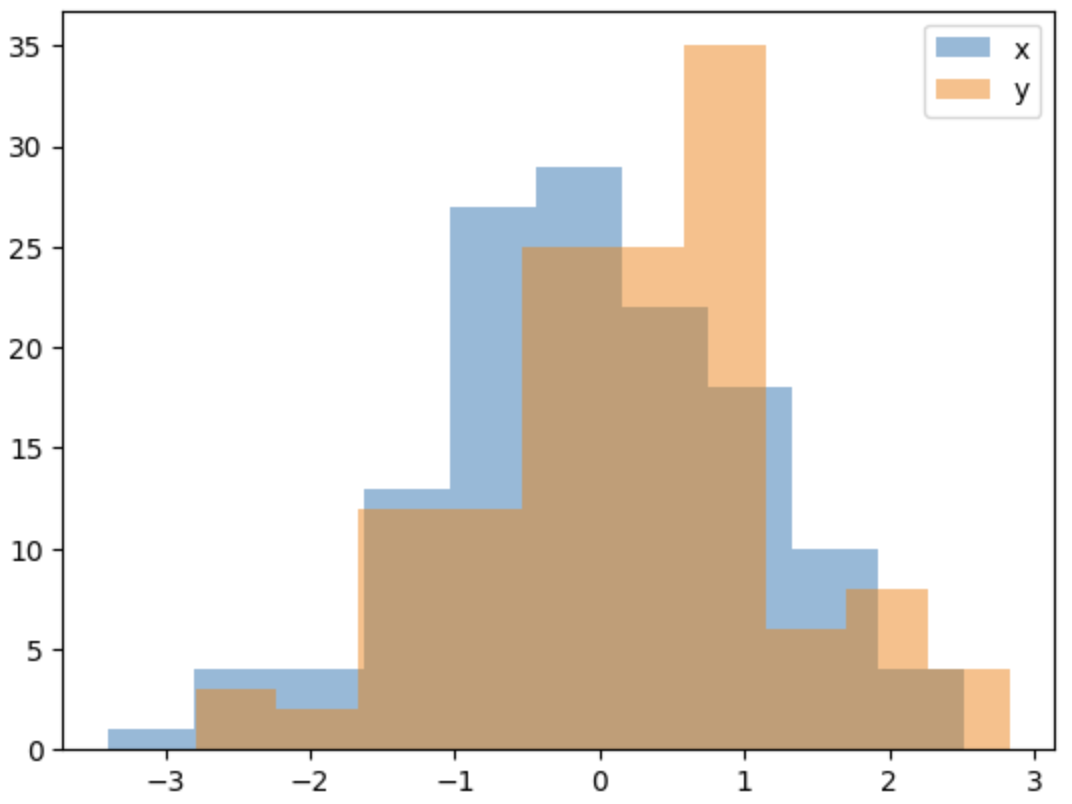
\includegraphics[width=0.75\textwidth]{images/5.png}
	\end{center}
	\caption{Выборки в момент, когда гипотеза была отвергнута}
	\label{img:5}
\end{figure}

\clearpage
